\documentclass[10pt,twocolumn]{article}
\usepackage[margin=0.72in,columnsep=0.24in]{geometry}
\usepackage{booktabs}
\usepackage{graphicx}
\usepackage{amsmath}
\usepackage{hyperref}
\usepackage{xcolor}

\title{When Circuit Structure Transfers: Wire-Dependency DAGs for Size-Generalizing Quantum Compiler Models}

\author{Anonymous Authors \\ Affiliation withheld for review}

\begin{document}
\maketitle

\begin{abstract}
Learned quantum-circuit models are commonly evaluated on circuits drawn from the same size distribution as training, leaving unclear whether their representation preserves the semantics needed at larger scales. We compare a wire-dependency directed acyclic graph (DAG) message-passing network with a parameter-matched canonical layer-grid recurrent model on depth-critical gate prediction. Both models receive identical gate, operand-role, wire-membership, and angle features and identical optimization budgets. Across three frozen paired seeds, training on 4--8-qubit, 24--56-gate circuits and testing on 9--12-qubit, 64--96-gate circuits, the DAG improves AUROC from 0.7861 to 0.8078 and F1 from 0.6055 to 0.6341. The DAG wins every paired seed and is equivariant to legal topological reorderings. The result reverses in distribution: the grid reaches 0.9406 AUROC versus 0.8556 for the DAG. Two downstream rewrite-ranking studies show the boundary of this advantage. The DAG consistently improves controlled identity-rewrite prioritization but misses a predeclared effect-size gate; on a routed structured-circuit development benchmark, the grid remains stronger. We conclude that explicit dependency structure improves size transfer for circuit reasoning, while practical optimization benefit requires richer hardware-aware objectives. Code, frozen protocols, negative results, and machine-readable records accompany the submission.
\end{abstract}

\section{Introduction}

Quantum compilation operates on objects with two simultaneous organizations. A circuit has a serialized or layered presentation, but its semantics and scheduling constraints are induced by dependencies along qubit wires. A gate may move across operations on disjoint wires without changing the circuit. Circuit width and length also vary substantially between small training examples and useful workloads. These properties create a representation question for quantum machine learning: should a model learn from a canonical grid, or should the dependency relation be explicit?

This question matters because near-term quantum workflows are constrained by circuit depth, two-qubit gates, routing overhead, and limited hardware connectivity \cite{preskill2018nisq,li2019tackling,cowtan2019qubit}. A representation that fits familiar circuit sizes can still fail when the number of wires or gates changes. Conversely, graph message passing supplies an inductive bias for relational structure \cite{gilmer2017mpnn,kipf2017gcn}, but that bias can reduce capacity to memorize regular positions. An empirical comparison therefore needs both in-distribution and size-shifted evaluation.

We study depth-critical gate prediction: identify gates that lie on at least one maximum-length path in the wire-dependency DAG. This task isolates whether a learned representation can propagate scheduling information. Labels are exact, allowing us to separate representation behavior from noisy supervision. The task is diagnostic rather than a replacement for the linear-time critical-path algorithm.

Our contributions are:
\begin{itemize}
    \item A matched comparison between a six-layer wire-dependency DAG network and a canonical earliest-layer bidirectional recurrent grid, with 87,745 and 88,417 parameters respectively.
    \item A frozen three-seed size-transfer experiment showing a consistent DAG advantage on circuits wider and longer than training, alongside a clear grid advantage in distribution.
    \item An equivariance test showing DAG logits are unchanged to within $10^{-6}$ under legal topological reordering.
    \item Two downstream rewrite-ranking studies, including failed confirmatory gates, that delimit what the representation result does and does not establish.
    \item Reproducible protocols, deterministic data generation, hashes, tests, compute records, and retained negative development trials.
\end{itemize}

\section{Circuit representations}

Let a circuit contain ordered operations $V=\{v_i\}_{i=1}^m$ on $n$ logical qubits. For each wire, we connect consecutive operations touching that wire. The union of these directed edges forms a DAG $G=(V,E)$. An edge carries the wire identity, while each node contains gate type, wire membership, control and target roles, and sine/cosine angle features. This construction preserves operand direction and does not connect operations that are independent.

The grid control first computes deterministic earliest dependency layers. Within a layer, gates are ordered by operands, gate type, and parameters. A bidirectional GRU processes the resulting canonical sequence. Canonicalization prevents arbitrary input serialization from becoming an uncontrolled weakness, giving the grid a strong deterministic ordering.

The DAG model projects node features to width 64 and applies six residual bidirectional message-passing blocks. Forward messages travel from predecessors and backward messages from successors; wire identity is concatenated to every message. A linear head emits one logit per operation. The grid uses width 96 and two bidirectional GRU layers. The resulting parameter counts differ by less than one percent.

The label for node $v$ follows exact dynamic programming. Let $f(v)$ be the longest predecessor path ending at $v$, $b(v)$ the longest successor path beginning at $v$, and $D=\max_v f(v)$. Then
\begin{equation}
y_v = \mathbf{1}[f(v)+b(v)-1=D].
\end{equation}
This label marks every operation on at least one maximum dependency path.

\section{Experimental design}

\subsection{Data and firewall}

Deterministic random circuits use H, RY, RZ, and directed CX gates. Training circuits have 4--8 qubits and 24--56 operations. The same-size test follows that range; the shifted test has 9--12 qubits and 64--96 operations. Training, validation, same-size test, reordered test, and larger test have distinct seeds and stored SHA-256 hashes. Development compared raw sequence, Transformer, canonical grid, fixed-depth DAG, and recurrent DAG variants. We froze the final architectures, data ranges, 6,000-update budget, metrics, and positive gate before generating final data.

Three paired training seeds (51--53) use identical data and update counts. AdamW optimization, batch construction, validation-only checkpoint selection, and node features are shared. We report node-level AUROC and F1. Means and sample standard deviations are across seeds.

\subsection{Predeclared claim}

The size-transfer claim required the DAG to beat the grid in larger-circuit AUROC for every seed, achieve a mean AUROC improvement of at least 0.015, and improve mean larger-circuit F1. Same-size superiority was not required. A separate implementation test randomly chooses legal topological orders and checks logit agreement.

\subsection{Downstream studies}

We ran two compiler-utility follow-ups. First, models ranked arbitrary single-gate deletions labeled by complete statevector fidelity. Second, they selected among exactly removable RZ$(0)$ identities, with utility measured by realized dependency-depth reduction. The second study used a frozen fresh 512-circuit test and three paired seeds.

We then built a development-only hardware-routing task using QAOA-like, hardware-efficient VQE, reversible arithmetic, and chemistry-inspired circuits. Candidates represented bound-zero removal, inverse-rotation cancellation, and self-inverse CNOT cancellation. Every candidate passed exact statevector verification. Exhaustive Qiskit compilation to a line coupling graph supplied routed CX and depth utility. The learned ranker received one candidate choice. This benchmark underwent a metric correction and two recorded development revisions before its stop rule; no final test was opened because the DAG development gate failed.

\section{Results}

\begin{figure}[t]
\centering
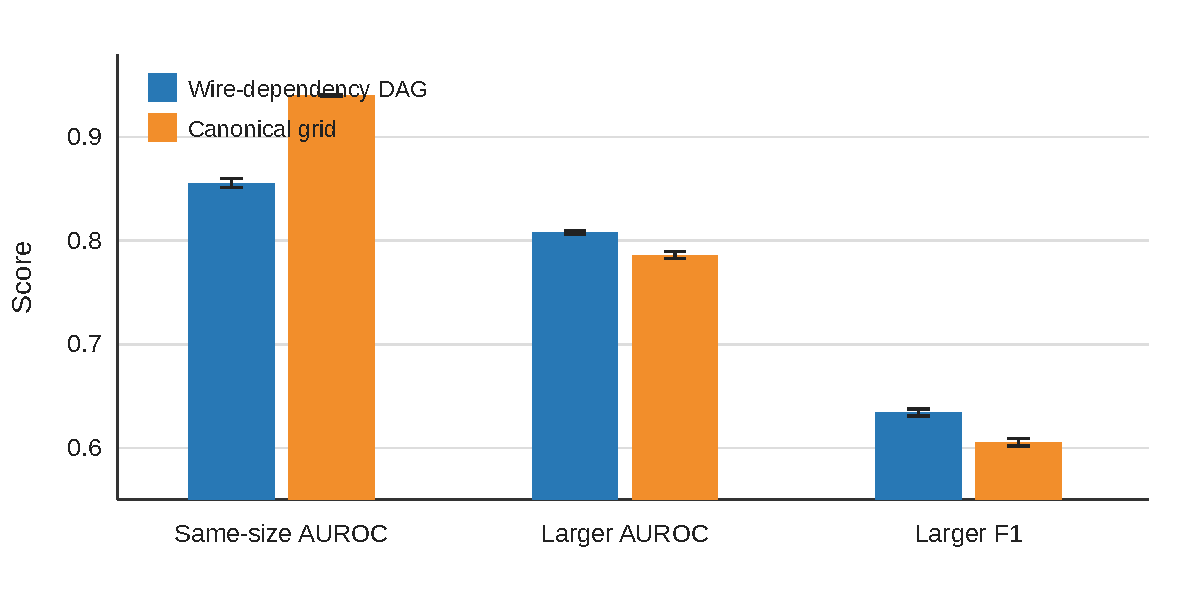
\includegraphics[width=\columnwidth]{figures/results.pdf}
\caption{Representation behavior reverses under circuit-size shift. Error bars show sample standard deviation across three paired seeds.}
\label{fig:main}
\end{figure}

\begin{table}[t]
\centering
\caption{Frozen three-seed critical-gate results (mean $\pm$ sample standard deviation).}
\label{tab:main}
\resizebox{\columnwidth}{!}{%
\begin{tabular}{lccc}
\toprule
Encoding & Same AUROC & Larger AUROC & Larger F1\\
\midrule
DAG & $0.8556\pm.0042$ & $\mathbf{0.8078\pm.0015}$ & $\mathbf{0.6341\pm.0033}$\\
Grid & $\mathbf{0.9406\pm.0008}$ & $0.7861\pm.0035$ & $0.6055\pm.0037$\\
\bottomrule
\end{tabular}}
\end{table}

Table~\ref{tab:main} and Fig.~\ref{fig:main} show a representation reversal. The grid dominates on familiar sizes by 0.0850 AUROC, suggesting that deterministic layer positions are highly learnable in distribution. On larger circuits, the DAG wins every seed. Paired AUROC improvements are 0.0202, 0.0177, and 0.0274, with mean 0.0217. The paired F1 improvement is 0.0286. Descriptive seed-level 95\% $t$ intervals are [0.0093, 0.0342] for AUROC difference and [0.0219, 0.0353] for F1 difference; with only three seeds, these intervals should not be read as strong asymptotic inference.

Legal topological reordering changes DAG logits by less than $10^{-6}$. Canonical-grid output also remains stable because the grid explicitly re-canonicalizes the circuit. A raw sequence model does not: in development, its AUROC fell under reordering and reached only 0.7303 on larger circuits, compared with 0.7687 for the canonical grid and 0.7933 for the selected DAG at the corresponding development stage. A token Transformer and recurrent DAG were also weaker development controls. These trials guided architecture selection and are not final-test evidence.

\begin{table}[t]
\centering
\caption{Downstream rewrite evidence. ``Passed'' refers to each frozen gate.}
\label{tab:downstream}
\resizebox{\columnwidth}{!}{%
\begin{tabular}{lccc}
\toprule
Study & DAG & Grid & Passed\\
\midrule
Safe deletion, one-call success & .9688 & 1.0000 & No\\
Identity rewrite, oracle depth recovered & .5194 & .4815 & No\\
Routed rewrite dev., mean CX reduction & 6.305 & 6.664 & No\\
\bottomrule
\end{tabular}}
\end{table}

The deletion task was saturated by a smallest-angle heuristic, which achieved perfect one-call success. In controlled identity ranking, DAG recovered 51.94\% of oracle depth reduction versus 48.15\% for grid and 17.93\% for random. DAG won all three paired seeds, but its 3.79-point mean advantage missed the predeclared 5-point gate. The routed structured-circuit development benchmark also failed to establish a DAG advantage: the final candidate-aware revision removed 6.305 CX gates on average versus 6.664 for grid. Both learned methods exceeded exact source criticality (3.266), while DAG exceeded source-depth lookahead (5.383). We did not open a final routed test.

\section{Discussion}

The results support a narrow mechanism. A grid can exploit stable positions when train and test sizes match. Width and length shifts change those positions and the number of recurrent steps. DAG messages instead follow wire dependencies whose meaning persists across sizes. Fixed-depth message passing does not solve critical path exactly, yet it retains useful local dependency patterns under the tested shift.

This finding does not imply that DAGs universally improve quantum-circuit learning. The grid is substantially better in distribution and remains stronger on the routed development endpoint. It also does not justify replacing exact scheduling algorithms with a neural network. Critical-path prediction is a controlled probe of representation transfer. A practical learned compiler should predict a cost that is expensive to obtain directly, such as post-routing performance under many candidate rewrites, calibrated noise-aware utility, or downstream synthesis interactions.

The failed downstream studies are informative. Small rotations create a trivial fidelity shortcut. Injected identities remove that shortcut but remain synthetic. Hardware routing creates an expensive objective, yet the canonical grid performs better in development. Better structural generalization on one diagnostic therefore does not automatically translate into optimization advantage.

\section{Limitations and reproducibility}

Circuits in the confirmatory study are synthetic and contain at most 12 qubits. Only three final training seeds were run. The exact labels make the diagnostic clean but algorithmically solvable. Hyperparameter budgets are matched rather than exhaustively optimized per model. The DAG is derived from a native PyTorch reimplementation; runtime parity with the original DGL code is not claimed. The routed benchmark uses a line coupling map and Qiskit optimization level 0 and remains development-only.

The repository stores every protocol before its corresponding final result, deterministic generators, split hashes, model parameter counts, training histories, machine-readable metrics, failed trials, and a compute ledger. Twenty-eight tests cover gate semantics, canonical scheduling, graph aggregation, topological equivariance, fidelity labels, rewrite utility, and exact rewrite templates. No GPU or paid resource was used.

\section{Conclusion}

Explicit wire-dependency message passing improves transfer of depth-critical reasoning from small to wider and longer quantum circuits, while a canonical grid is much stronger on familiar sizes. The reversal demonstrates that in-distribution accuracy alone can select the wrong representation for scalable circuit reasoning. Downstream experiments do not yet establish production compiler benefit. Future work should test public circuit suites, more seeds and widths, multiple hardware graphs, graph-transformer controls, and expensive hardware-aware objectives where amortized prediction can replace repeated compilation.

\bibliographystyle{unsrt}
\bibliography{references}
\end{document}
